\documentclass[main.tex]{subfiles}

\begin{document}

\section{Лекция 20.12.2023}

Я лекцию, к сожалению, пропустил. ОРВИ/ОРЗ.

На занятии обсуждалась система времён английского глагола (tenses and aspects).

\subsection{Present Simple. Present Continuous}
\vspace{-10mm}
{\parindent-20pt\includegraphics[width=\textwidth, page=1,trim={0.25in 3in 0.25in 0.25in},clip=true]{TensesAndAspects.pdf}}\newpage

\subsection{Past Simple. Past Continuous}
\vspace{-5mm}
{\parindent-20pt\includegraphics[width=\textwidth, page=2,trim={0.25in 1in 0.25in 0.3in},clip=true]{TensesAndAspects.pdf}}\newpage

\subsection{Present Perfect. Present Perfect Continuous}
\vspace{-5mm}
{\parindent-20pt\includegraphics[width=\textwidth, page=3,trim={0.25in 1in 0.25in 0.3in},clip=true]{TensesAndAspects.pdf}}\newpage

\subsection{Past Perfect. Past Perfect Continuous. Simple Future (will)}
\vspace{-5mm}
{\parindent-20pt\includegraphics[width=\textwidth, page=4,trim={0.25in 1in 0.25in 0.5in},clip=true]{TensesAndAspects.pdf}}\newpage

\subsection{To be going to. Future Continuous. Future Perfect. Future Perfect Continuous}
\vspace{-5mm}
{\parindent-20pt\includegraphics[width=\textwidth, page=5,trim={0.25in 1in 0.25in 0.85in},clip=true]{TensesAndAspects.pdf}}\newpage

{\parindent-20pt\includegraphics[width=\textwidth, page=6,trim={0.25in 9in 0.25in 0.25in},clip=true]{TensesAndAspects.pdf}}

\subsection{VOICES. TENSES. ASPECTS}

{\parindent0pt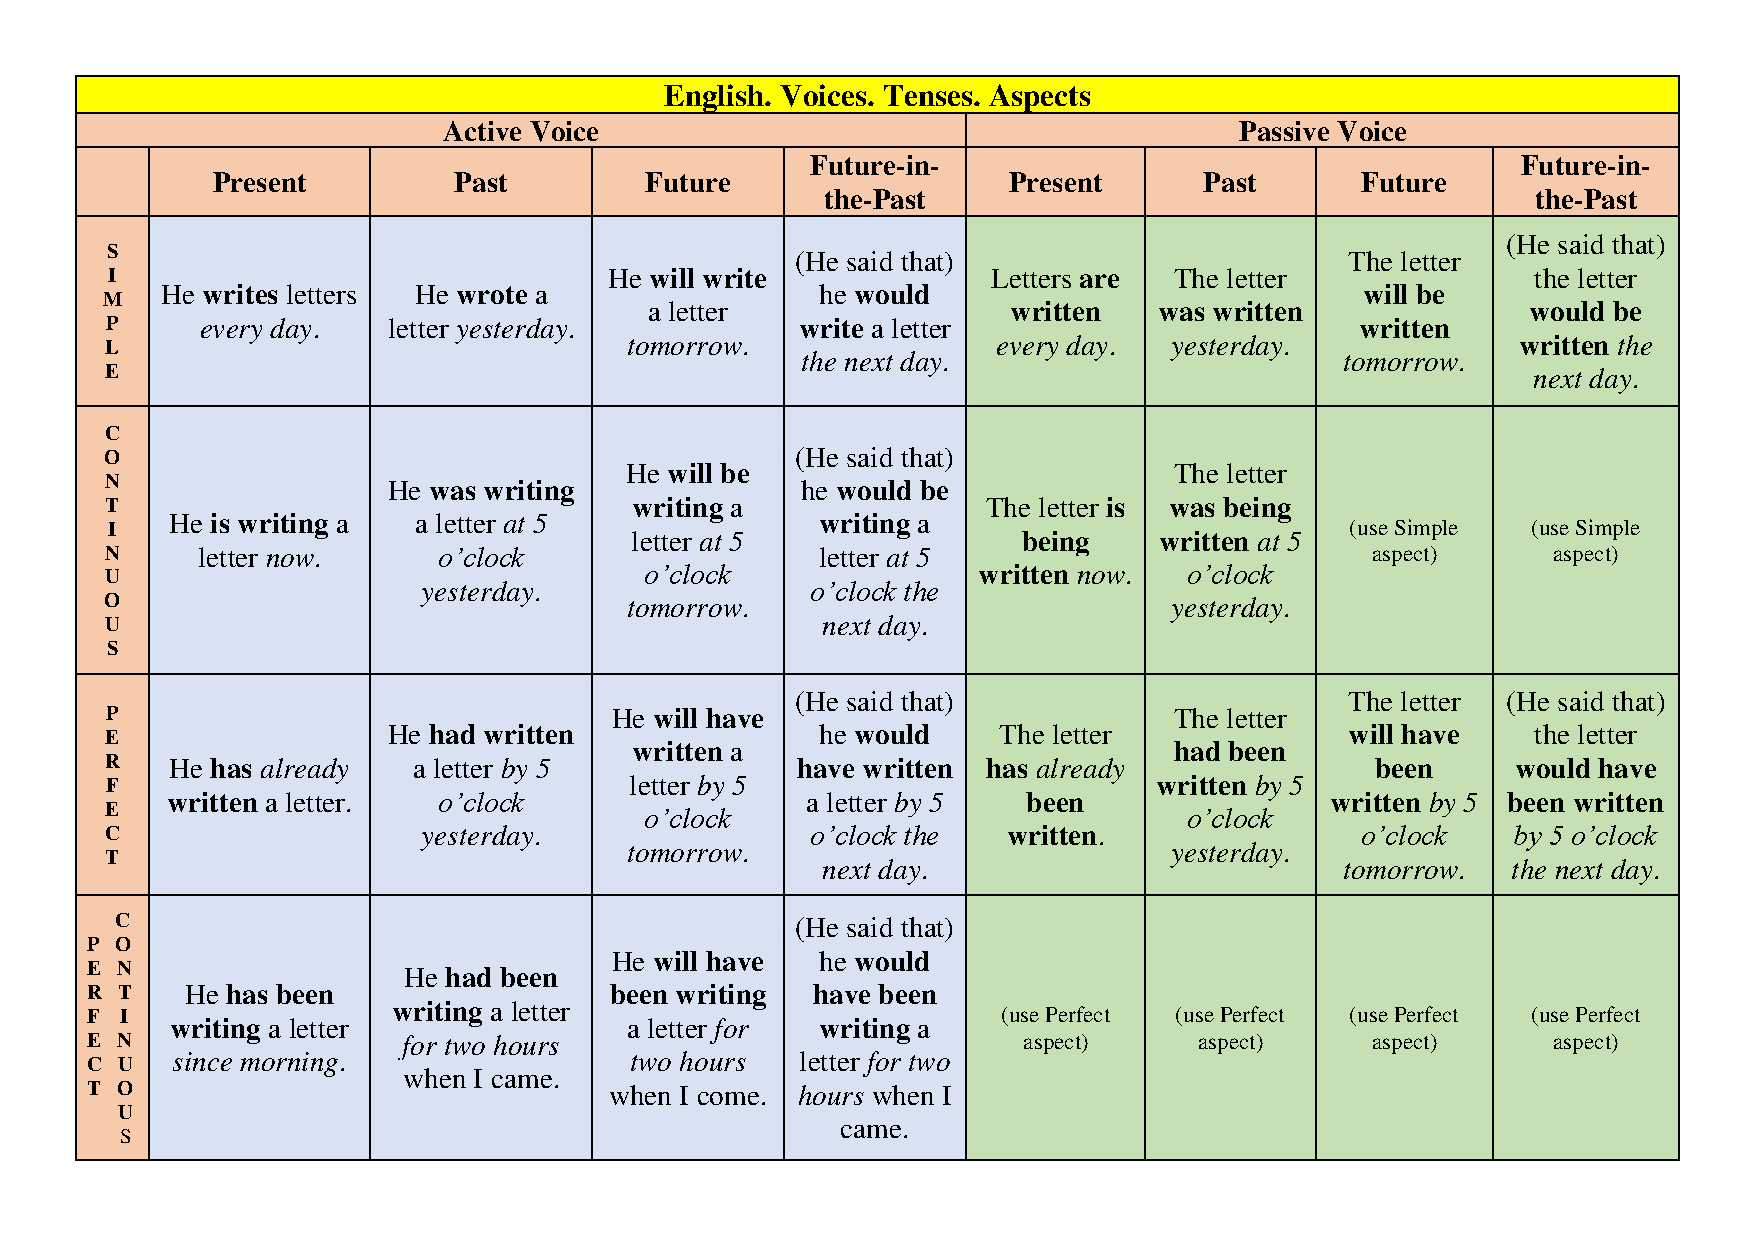
\includegraphics[width=\textwidth,page=1,trim={0.5in 0in 0.49in 0in},clip=true]{EnglishTensesAspectsVoicesPoster.pdf}}

\subsection{PASSIVE VOICE}

{\parindent-10pt\includegraphics[width=\textwidth, page=1,trim={0.6in 1.4in 0.26in 0.95in},clip=true]{PassiveVoice.pdf}}\newpage

\end{document}
